\subsection{Progettazione architetturale}
\label{progettazione_architetturale}
\textbf{Durata:} dal 2021\_02\_01 al 2021\_03\_01\\
La progettazione architetturale inizia appena concluso il periodo precedente e termina con la \glo{\textbf{RP}}.
Le precondizioni sono:
\begin{itemize}
    \item Le postcondizioni del periodo precedente sono state soddisfatte;
    \item La candidatura del gruppo al progetto {\NomeProgetto} è stata accolta.
\end{itemize}
Le postcondizioni sono:
\begin{itemize}
    \item Aggiornamento e correzione dei documenti già prodotti;
    \item Produzione del \glo{\textbf{Proof of concept}} e dell'\textbf{allegato tecnico};
    \item Completamento della progettazione ad alto livello del software;
    \item Consegna dei documenti richiesti in entrata alla \textbf{RP};
    \item Ultimata preparazione della presentazione da esporre in sede di revisione.
\end{itemize}
Le attività da svolgere durante il periodo sono:
\begin{itemize}
    \item \textbf{Incremento e verifica (dal 2021\_02\_01 al 2021\_02\_11):} i documenti già prodotti vengono migliorati e aggiornati se necessario ({\NdP}, {\PdP}, {\Glossario}, {\PdQ}, {\AdR});
    \item \glo{\textbf{Technology Baseline}} e \textbf{PoC}: viene fatta un'analisi ad alto livello del software e viene redatto l'Allegato tecnico dove vengono individuati i \glo{design pattern} che verranno adottati per lo sviluppo. Infine viene codificato il Proof of concept, il quale viene presentato o condiviso al committente e proponente in una data da definirsi. Il gruppo ipotizza di riuscire a sviluppare il Proof of concept attraverso due incrementi:
    \begin{itemize}
    	\item \textbf{Incremento 1 (dal 2021\_02\_10 al 2021\_02\_20)}: In questo periodo l'obiettivo principale è riuscire a implementare i requisiti e i casi d'uso fondamentali concordati con il proponente sotto forma di codice;
        \item \textbf{Incremento 2 (dal 2021\_02\_21 al 2021\_02\_27)}: Realizzazione dei requisiti e dei casi d'uso non completati precedentemente e miglioramento di quelli già implementati.
    \end{itemize}
\end{itemize}
\newpage
\subsubsection{Diagramma di Gantt: Progettazione architetturale}
\begin{figure}[ht]
    \centering
    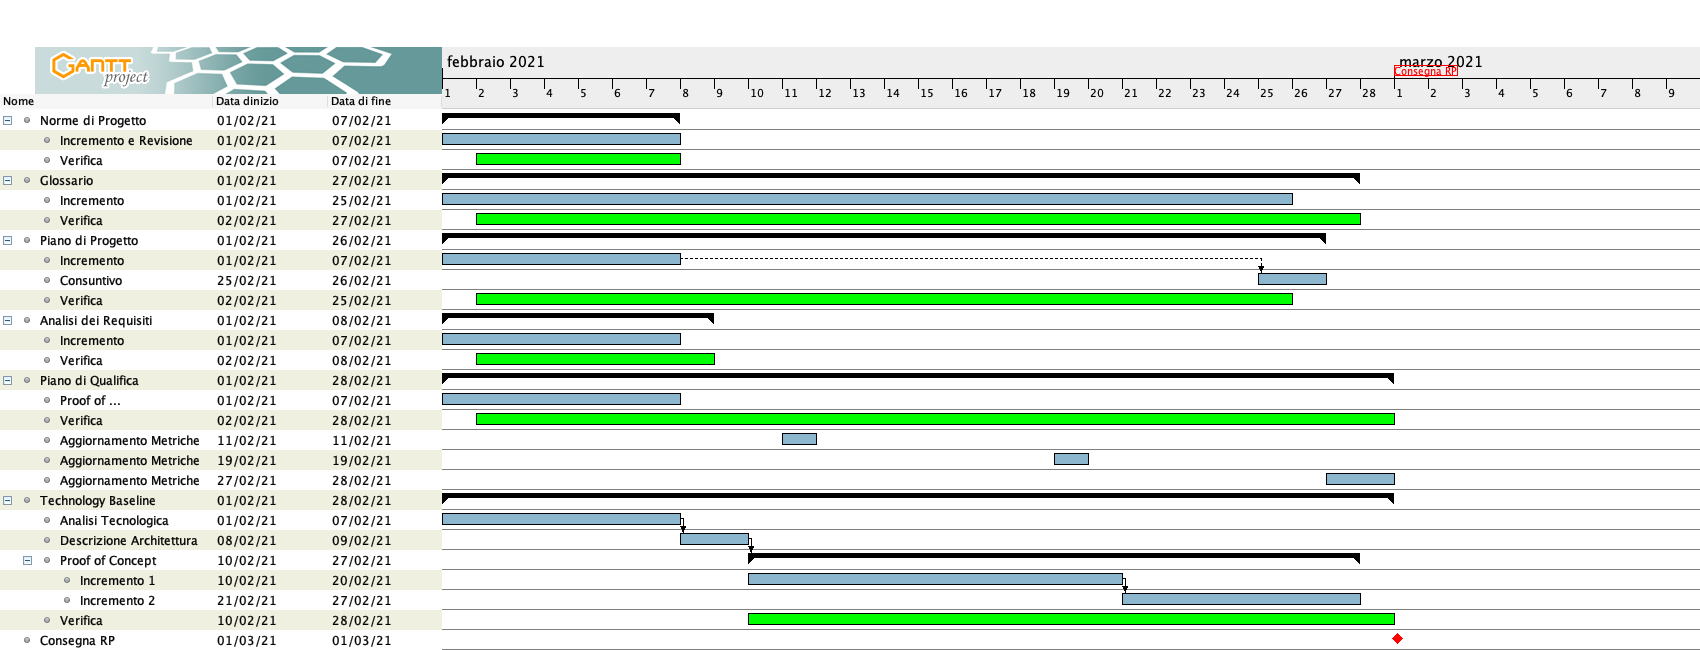
\includegraphics[width=\textwidth]{Immagini/GanttProgettazioneArchitetturale}
    \caption{Diagramma di Gantt dell'attività di progettazione architetturale}
\end{figure}